\chapter{龙芯新增多媒体指令}\label{chp:simd}

龙芯的多媒体指令扩展通过增加新的指令和新的 64 位数据类型
来提高多媒体及通信应用的表现。
新增加的指令集没有增加任何新的操作模型或者需要操作系统维护的
状态,保持了与现有龙芯平台上软硬件的兼容性。

现在多媒体、通信、以及图像软件大量地使用在较小的
数据元素上进行多层重复操作的复杂算法(iterative algorithms)。
龙芯的多媒体指令就是为了这个需求而产生的。比如,多数声音处理程序通常使用 16
位数据,而视频和图像软件 则多采用 8 位数据。龙芯的多媒体指令
采用了单指令多数据(single insruction multiple data,简称
SIMD)技术,用于提高软件并行处理多个数据元素的能力。

龙芯多媒体技术支持在 64 位上的字节,半字,字和双字元素的并行处理。
多媒体指令为每 64 位数据引入了新的包(Packed)数据类型。 包数据类型有如下
几类:
\begin{itemize}
  \item 字节包:字节是一个  8 位的数据结构, 每个字节包是 8 个连续字节的集合;
  \item 半字包:半字是一个 16 位的数据结构, 每个半字包是 4 个连续半字的集合;
  \item   字包:  字是一个 32 位的数据结构, 每个字包  是 2 个连续字的集合;
  \item 双字包:双字是一个 64 位的数据结构, 每个双字包就是一个 64 位的双字。
\end{itemize}
包内的单个数据元素都是整数类型,但可能有两种格式保存:无符号和有符号。
对每个单独的元素,数据存放的规则是:较低位存放数据低位,较高位存放数据高位。
每个数据元素也有它对应的最低位(leset significant bit,简称 LSB),和最高位
(most significant bit,简称 MSB)。图~\ref{fig:packed-data} 给出了这四种
无符号包的数据格式;有符号包有类似的格式,不同的是每个数据元素的最高位
被作为符号位。

\begin{figure}[htbp]
  \centering
  \setlength\fboxsep{10pt}
  \setlength\fboxrule{.5pt}
  \fbox{\scalebox{.78}{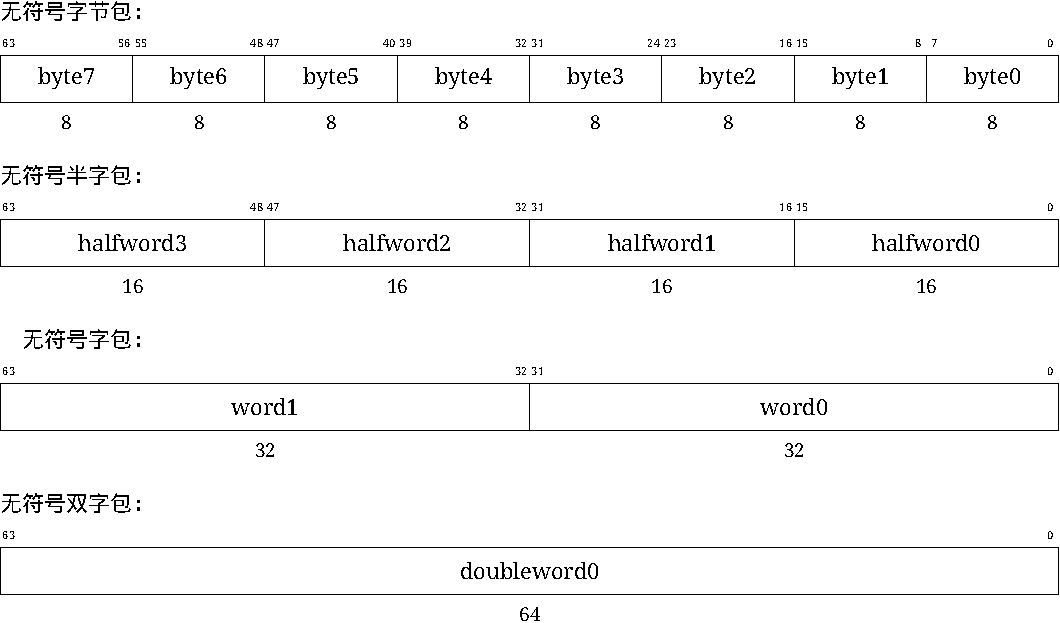
\includegraphics{packeddata-cn}}}
  \caption{无符号数据包格式}
  \label{fig:packed-data}
\end{figure}

在龙芯 GS464 处理器核上, 多媒体指令的编码是通过对 MIPS 指令的 协处理器 2
(CP2)指令进行自定义而实现的, 所以执行这些指令时要求协处理器 2 可用,即 CP0
的 Status 寄存器的 CU[2] 必须使能, 其中浮点相关指令还要求协处理器 1 可用。

\section{多媒体指令特性}

\subsection{饱和模式和截断模式}

当执行整数运算时,尤其是当数据元素的位数比较少的时候,运算结果很容易
超出可以表达的范围而导致不能保存。例如,当有符号半字整数运算,可能
会出现结果溢出,即最后结果大于 16 位可以存储的范围。当这种情况发生时,
龙芯的多媒体指令提供了三种处理超出范围的方法。它们分别是:
\begin{itemize}
  \item 截断模式

    截断模式是简单地将超出范围的结果截断,即溢出位都被忽略,只有有效的低位被
    保留,并存入目的。使用截断模式的应用程序应当控制操作数的范围,以防止超出
    范围的现象发生。如果操作数的范围不加以控制,截断模式
    可能产生较大的误差。例如,两个大的有符号数相加,如果产生
    正向的溢出。在截断模式下,结果可能是负数。

  \item 有符号饱和模式

    有符号饱和模式是在溢出发生时,尽可能的在有符号数的范围去表达超出范围的
    结果。例如,当有符号半字整数运算时,如果正向的溢出发生,那么结果将会被
    ``饱和''到 7FFFH --- 因为这是在 16 位的范围内能表达的最大整数。同理,如果,
    负向溢出发生,那么结果为 8000H,即最小的半字整数。

  \item 无符号饱和模式

    无符号饱和模式与有符号饱和模式类似, 它的思想是在溢出发生时,
    在无符号数的范围内尽量地表达溢出的无符号数。因此,当上溢发生时,
    无符号字节整数的结果为 FFH, 而下溢的结果会被饱和为 00H。其他数据类型
    同理可得。
\end{itemize}

一般而言,饱和模式在算术溢出的情况下,会给出更自然的结果。比如,
在色彩的计算中,饱和模式将会使得颜色结果为纯黑或纯白色(最大或最小值)
而不会出现颜色反转的情况。 当不可能检查源操作数范围时,
它还同时可以避免计算由于截断的原因出现奇怪的结果。

龙芯的多媒体指令不会因为计算中出现上溢或下溢的情况而触发例外。

\subsection{多媒体指令列表及格式}

多媒体指令的操作对象有以下几种不同情况:
\begin{itemize}
  \item 数据类型: 字节包, 半字包,字包,或者双字包?
  \item 符号位: 有符号或无符号数?
  \item 溢出控制: 饱和或截断模式?
\end{itemize}

\begin{table}[htbp]
  \centering
  \begin{tabular}{|>{\centering}p{2cm}|*{4}{>{\centering}p{3cm}|}} \hline
         & \multicolumn{4}{c|}{FUNC} \tabularnewline \cline{2-5}
             & ADD     & SUB     & MUL      & DIV \tabularnewline[-.2cm]
         fmt & 000000  & 000001  & 000010   & 000011 \tabularnewline \hhline
         24  & PADDSH  & PSUBSH  & PSHUFH   & PUNPCKLHW \tabularnewline
         25  & PADDUSH & PSUBUSH & PACKSSWH & PUNPCKHHW \tabularnewline
         26  & PADDH   & PSUBH   & PACKSSHB & PUNPCKLBH \tabularnewline
         27  & PADDW   & PSUBW   & PACKUSHB & PUNPCKHBH \tabularnewline
         28  & PADDSB  & PSUBSB  & PXOR     & PINSRH\_0 \tabularnewline
         29  & PADDUSB & PSUBUSB & PNOR     & PINSRH\_1 \tabularnewline
         30  & PADDB   & PSUBB   & PAND     & PINSRH\_2 \tabularnewline
         31  & PADDD   & PSUBD   & PANDN    & PINSRH\_3 \tabularnewline \hhline
             & ROUND.L & TRUNC.L & CEIL.L   & FLOOR.L \tabularnewline[-.2cm]
         fmt & 001000  & 001001  & 001010   & 001011 \tabularnewline \hhline
         24  & PAVGH   & PCMPEQW & PSLLW    & PSRLW \tabularnewline
         25  & PAVGB   & PCMPGTW & PSLLH    & PSRLH \tabularnewline
         26  & PMAXSH  & PCMPEQH & PMULLH   & PSRAW \tabularnewline
         27  & PMINSH  & PCMPGTH & PMULHH   & PSRAH \tabularnewline
         28  & PMAXUB  & PCMPEQB & PMULUW   & PUNPCKLWD \tabularnewline
         29  & PMINUB  & PCMPGTB & PMULHUH  & PUNPCKHWD \tabularnewline \hhline
             & ROUND.W & TRUNC.W & CEIL.W   & FLOOR.W \tabularnewline[-.2cm]
         fmt & 001000  & 001001  & 001010   & 001011 \tabularnewline \hhline
         24  & PADDU   & PSUBU   & PSLL     & PSRL \tabularnewline
         25  & POR     & PASUBUB & PDSLL    & PDSRL \tabularnewline
         26  & PADD    & PSUB    & PEXTRH   & PSRA \tabularnewline
         27  & PDADD   & PDSUB   & PMADDHW  & PDSRA \tabularnewline
         28  & PSEQU   & PSLTU   & PSLEU    & BIADD \tabularnewline
         29  & PSEQ    & PSLT    & PSLE     & PMOVMSKB \tabularnewline \hline
  \end{tabular}
  \caption{龙芯多媒体指令集}
  \label{tab:simd-ins}
\end{table}

表~\ref{tab:simd-ins} 列出了所有龙芯 GS464 新增的多媒体指令。
通常,多媒体指令采用如下的格式:
\begin{itemize}
  \item 前缀: P 表示指令操作包数据类型;
  \item 中段: 具体指令, 如 ADD,CMP,或 XOR 等;
  \item 后缀
    \begin{itemize}
      \item US: 无符号,饱和;
      \item S: 有符号,饱和;
      \item B,H,W,D: 数据类型 --- 分别表示 字节包(byte),
        半字包(halfword), 字包(word), 或双字包(doubleword)。
    \end{itemize}
\end{itemize}

如果一条指令有不同的输入和输出结果类型时,那么它将会有两个数据类型的后缀。
比如说,转换指令将一种包类型数据转换为另一种包数据类型,那么它有两个数据类型
后缀:第一个是输入数据类型,而第二个是输出数据类型。以下是一条龙芯多媒体指令
的助记格式的实例:
\begin{verbatim}
   PADDUSW (无符号字整数饱和模式加)
   P   = 包数据
   ADD = 指令操作
   US  = 无符号饱和模式
   W   = 字
\end{verbatim}

\section{多媒体指令详解}

在以下的各小节中,将逐个对每个指令进行详细的介绍。

\subsection{PACKSSHB/PACKSSWH (有符号数打包)}

\begin{instructionblk}
  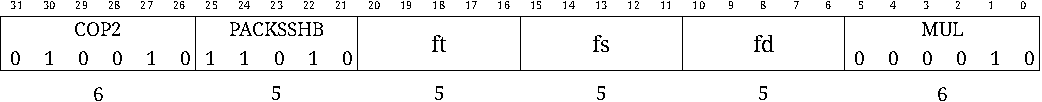
\includegraphics{ins-PACKSSHB} \\
  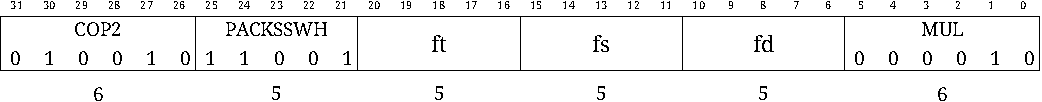
\includegraphics{ins-PACKSSWH} \\
  \instructionbody{PACK.SSHB fd,fs,ft \narrownewline PACK.SSWH fd,fs,ft}
  {饱和模式有符号数打包:将包结构转换为较窄的格式。}
  {PACKSSHB将有符号半字包转换用饱和模式转换为有符号字节包,而
  PACKSSWH将有符号字包转换用饱和模式转换为有符号半字包。
  共同特点是使用饱和条件转换较宽的数据类型到较窄的数据类型。

  PACKSSHB的具体操作是将``第一个操作数的4个有符号整数半字和
  第二个操作数的4个有符号半字整数'',共8个有符号整数半字,转换
  为8个有符号字节整数,并将结果存入目标操作数。转换的过程使用饱和模式:
  在转换过程中, 如果一个有符号半字整数的值超出一个有符号字节的整数范围
  (大于EFH或小于80H),则生成的的有符号字节整数分别为EFH或80H。
  
  PACKSSWH的操作类似,不同的是操作对象是有符号字整数,并生成有符号半字整数。}
  {PACKSSHB \narrownewline
  fd[ 7..0 ] $\leftarrow$ SaturateSignedHalfwordToSignedByte fs[15..0 ]; \narrownewline
  fd[15..8 ] $\leftarrow$ SaturateSignedHalfwordToSignedByte fs[31..16]; \narrownewline
  fd[23..16] $\leftarrow$ SaturateSignedHalfwordToSignedByte fs[47..32]; \narrownewline
  fd[31..24] $\leftarrow$ SaturateSignedHalfwordToSignedByte fs[63..48]; \narrownewline
  fd[39..32] $\leftarrow$ SaturateSignedHalfwordToSignedByte ft[15..0 ]; \narrownewline
  fd[47..0 ] $\leftarrow$ SaturateSignedHalfwordToSignedByte ft[31..16]; \narrownewline
  fd[55..48] $\leftarrow$ SaturateSignedHalfwordToSignedByte ft[47..32]; \narrownewline
  fd[63..56] $\leftarrow$ SaturateSignedHalfwordToSignedByte ft[63..48]; \narrownewline \narrownewline
  PACKSSWH \narrownewline
  fd[15..0 ] $\leftarrow$  SaturateSignedWordToSignedHalfWord fs[31..0 ]; \narrownewline
  fd[31..16] $\leftarrow$  SaturateSignedWordToSignedHalfWord fs[63..32]; \narrownewline
  fd[47..32] $\leftarrow$  SaturateSignedWordToSignedHalfWord ft[31..0 ]; \narrownewline
  fd[63..48] $\leftarrow$  SaturateSignedWordToSignedHalfWord ft[63..32];}
  {无。}
\end{instructionblk}


\subsection{PACKUSHB (无符号数打包)}

\begin{instructionblk}
  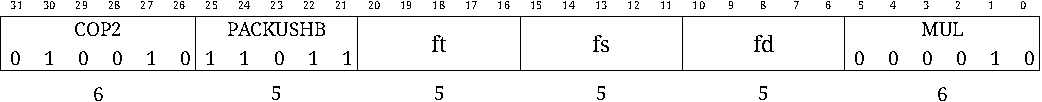
\includegraphics{ins-PACKUSHB} \\
  \instructionbody{PACKUSHB fd,fs,ft}
  {饱和模式无符号数打包}
  {PACKUSHB将有符号半字包转换用饱和模式转换为无符号字节包。
  具体的操作是将``第一个操作数的4个有符号整数半字和
  第二个操作数的4个有符号整数半字'',共8个有符号整数半字,转换
  为8个无符号字节整数,并将结果存入目标操作数。转换的过程使用饱和模式:
  在转换过程中, 如果一个有符号半字整数的值超出一个无符号字节的整数范围
  (大于FFH或小于00H),则生成的的无符号整数字节分别为FFH或00H。}
  {PACKUSHB \narrownewline
  fd[ 7..0 ] $\leftarrow$ SaturateSignedHalfwordToUnsignedByte fs[15..0 ]; \narrownewline
  fd[15..8 ] $\leftarrow$ SaturateSignedHalfwordToUnsignedByte fs[31..16]; \narrownewline
  fd[23..16] $\leftarrow$ SaturateSignedHalfwordToUnsignedByte fs[47..32]; \narrownewline
  fd[31..24] $\leftarrow$ SaturateSignedHalfwordToUnsignedByte fs[63..48]; \narrownewline
  fd[39..32] $\leftarrow$ SaturateSignedHalfwordToUnsignedByte ft[15..0 ]; \narrownewline
  fd[47..0 ] $\leftarrow$ SaturateSignedHalfwordToUnsignedByte ft[31..16]; \narrownewline
  fd[55..48] $\leftarrow$ SaturateSignedHalfwordToUnsignedByte ft[47..32]; \narrownewline
  fd[63..56] $\leftarrow$ SaturateSignedHalfwordToUnsignedByte ft[63..48];}
  {无。}
\end{instructionblk}


\subsection{PADDB/PADDH/PADDW/PADDD (整数包加)}


\begin{instructionblk}
  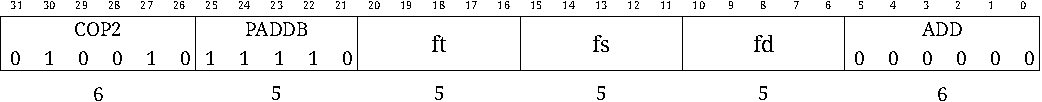
\includegraphics{ins-PADDB} \\
  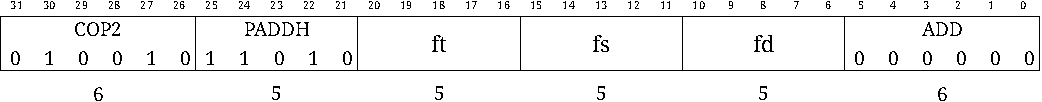
\includegraphics{ins-PADDH} \\
  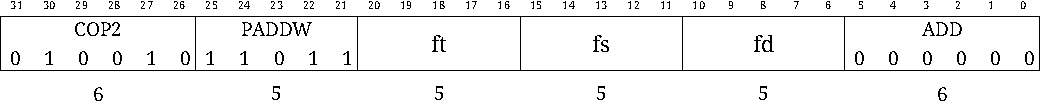
\includegraphics{ins-PADDW} \\
  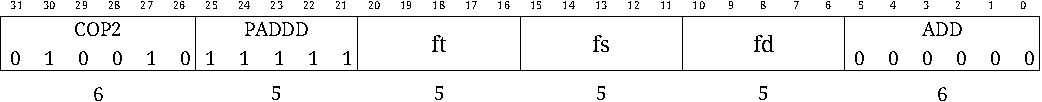
\includegraphics{ins-PADDD} \\
  \instructionbody{PADDB fd,fs,ft \narrownewline PADDH fd,fs,ft \narrownewline PADDW fd,fs,ft \narrownewline PADDD fd,fs,ft}
  {使用截断模式执行各种整数包类型相加运算。}
  {这四条指令用于执行各种整数包加法操作: 它们分别将第一个和第二个操作寄存器的
  对应位置的各个操作数(依照指令给定的数据类型)相加,并将结果存储在目标操作数中。
  溢出处理为截断模式。 比如说, PADDB指令的具体操作是将第一个和第二个操作寄存器
  对应的 8 个字节整数相加。当任何一个加法结果太大,即在第9位溢出时,只有低 8
  位结果将被写入到目标操作数(进位被忽略)。其他三个指令与PADDB类似。
  
  注意,这四条包加法指令既可以应用于无符号,也可以应用于(采用2的补码
  表示法的)有符号整数包。 为了避免溢出或进位情况的发生,软件必须控制操作数的范围。}
  {PADDB \narrownewline
  fd[ 7..0 ] $\leftarrow$ fs[ 7..0 ] + ft[ 7..0 ]; \narrownewline
  * repeat add operation for 2nd through 7th byte *; \narrownewline
  fd[63..56] $\leftarrow$ fs[63..56] + ft[63..56]; \narrownewline \narrownewline
  PADDH \narrownewline
  fd[15..0 ] $\leftarrow$ fs[15..0 ] + ft[15..0 ]; \narrownewline
  * repeat add operation for 2nd and 3th halfword *; \narrownewline
  fd[63..48] $\leftarrow$ fs[63..48] + ft[63..48]; \narrownewline \narrownewline
  PADDW \narrownewline
  fd[31..0 ] $\leftarrow$ fs[31..0 ] + ft[31..0 ]; \narrownewline
  fd[63..32] $\leftarrow$ fs[63..32] + ft[63..32]; \narrownewline \narrownewline
  PADDD \narrownewline
  fd[63..0 ] $\leftarrow$ fs[63..0 ] + ft[63..0 ];}
  {无。}
\end{instructionblk}

\subsection{PADDSB/PADDSH (有符号整数包加)}

\begin{instructionblk}
  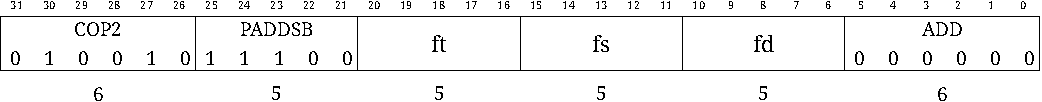
\includegraphics{ins-PADDSB} \\
  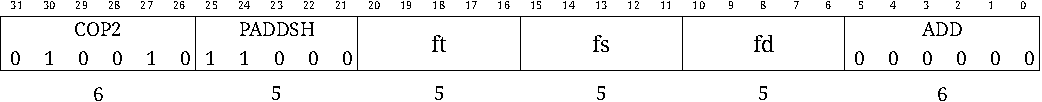
\includegraphics{ins-PADDSH} \\
  \instructionbody{PADDSB fd,fs,ft \narrownewline PADDSH fd,fs,ft}
  {有符号整数包加}
  {这两条指令用于执行各种有符号整数包的加法操作: 它们分别将第一个和第二个操作寄存器的
  对应位置的各个操作数(依照指令给定的数据类型)相加,并将结果存储在目标操作数中。
  溢出处理采用有符号饱和模式。 这些指令的操作数皆为 64 位。

  PADDSB指令的具体操作是将第一个和第二个操作寄存器
  对应的 8 个有符号字节整数相加。当任何一个加法结果太大或太小,
  超出了一个有符号字节的整数范围(即大于 7FH 或少于
  80H),则对应的饱和值7FH或80H,将被写入目的操作数。
  相应的, PADDSH指令操作有符号半字整数。当一个
  半字相加的结果超出了有符号半字整数范围时(即大于
  7FFFH或小于8000H),则7FFFH或8000H的作为饱和值,将写入目标操作数。}
  {PADDSB \narrownewline
  fd[ 7..0 ]  $\leftarrow$ SaturateToSignedByte(fs[ 7..0 ] + ft[ 7..0 ]); \narrownewline
  * repeat add operation for 2nd through 7th bytes *; \narrownewline
  fd[63..56] $\leftarrow$ SaturateToSignedByte(fs[63..56] + ft[63..56]); \narrownewline \narrownewline
  PADDSH \narrownewline
  fd[15..0 ] $\leftarrow$ SaturateToSignedHalfword(fs[15..0 ] + ft[15..0 ]); \narrownewline
  * repeat add operation for 2nd and 7th halfwords *; \narrownewline
  fd[63..48] $\leftarrow$ SaturateToSignedHalfword(fs[63..48] + ft[63..48]);}
  {无。}
\end{instructionblk}

\subsection{PADDUSB/PADDUSH (无符号整数包加)}

\begin{instructionblk}
  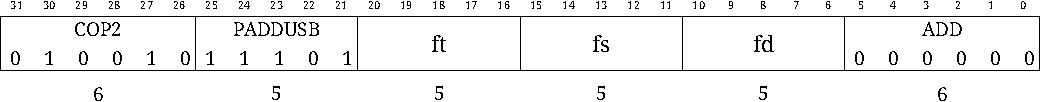
\includegraphics{ins-PADDUSB} \\
  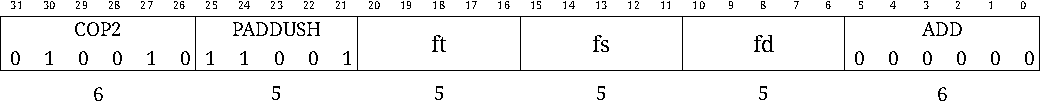
\includegraphics{ins-PADDUSH} \\
  \instructionbody{PADDUSB fd,fs,ft \narrownewline PADDUSH fd,fs,ft}
  {无符号整数包加法运算。}
  {这两条指令用于执行各种无符号整数包加操作: 它们分别将第一个和第二个操作寄存器的
  对应位置的各个操作数(依照指令给定的数据类型)相加,并将结果存储在目标操作数中。
  溢出处理采用无符号饱和模式。

  PADDUSB指令的具体操作是将第一个和第二个操作寄存器
  对应的 8 个无符号字节整数相加。当任何一个加法结果太大,
  超出了一个无符号字节的整数范围(即大于 FFH),
  则FFH将作为饱和值写入目的操作数。
  相应的, PADDUSH指令操作无符号半字整数。当一个
  半字相加的结果超出了无符号半字整数范围时(即大于
  FFFFH),则FFFFH作为饱和值将写入目标操作数。}
  {PADDUSB \narrownewline
  fd[ 7..0 ]  $\leftarrow$ SaturateToUnsignedByte(fs[ 7..0 ] + ft[ 7..0 ]); \narrownewline
  * repeat add operation for 2nd through 7th bytes *; \narrownewline
  fd[63..56] $\leftarrow$ SaturateToUnsignedByte(fs[63..56] + ft[63..56]); \narrownewline \narrownewline
  PADDUSH \narrownewline
  fd[15..0 ] $\leftarrow$ SaturateToUnsignedHalfword(fs[15..0 ] + ft[15..0 ]); \narrownewline
  * repeat add operation for 2nd and 3rd halfwords *; \narrownewline
  fd[63..48] $\leftarrow$ SaturateToUnsignedHalfword(fs[63..48] + ft[63..48]);}
  {无。}
\end{instructionblk}

\subsection{PANDN (逐位逻辑与非)}

\begin{instructionblk}
  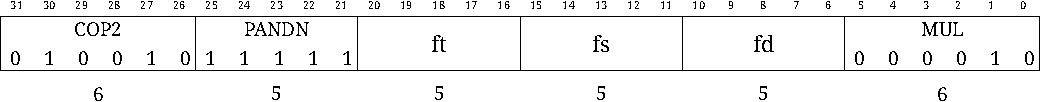
\includegraphics{ins-PANDN} \\
  \instructionbody{PANDN fd,fs,ft}
  {逐位逻辑与非操作}
  {该指令执行逐位逻辑与非操作。 具体操作为,首先对第一个操作数进行按位非逻辑
  运算,然后将结果和第二个操作数进行按位逻辑与运算, 并将结果写入
  目标操作数。所有源和目的操作数都是 64 位寄存器。}
  {PANDN \narrownewline
  fd$\leftarrow$(NOT fs) AND ft;}
  {无。}
\end{instructionblk}

\subsection{PAVGB/PAVGH (无符号整数包求平均)}

\begin{instructionblk}
  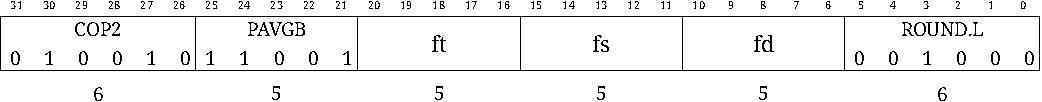
\includegraphics{ins-PAVGB} \\
  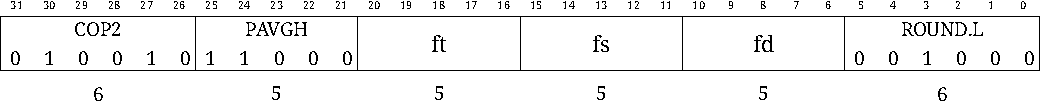
\includegraphics{ins-PAVGH} \\
  \instructionbody{PAVGB fd,fs,ft \narrownewline PAVGH fd,fs,ft}
  {包整数求平均值}
  {这两条指令执行无符号整数包求平均操作: 对第一个操作数和第二个操作数
  对应位置的无符号整数求平均,并将结果存储在目标操作数中。在操作中,当第一个操作数
  中的元素和第二个操作数中的对应元素相加时,其和还被加 1,然后结果右移一位(除2操作)。
  注意,加1的操作的实质效果是使得求平均结果为四舍五入。
  所有的源和目的操作数皆是64位寄存器。

  PAVGB指令用于无符号字节整数包, 而PAVGH用于无符号半字整数包。}
  {PAVGB \narrownewline
  * temp sum before shifting is 9 bits * \narrownewline
  ft[ 7..0 ] $\leftarrow$ (fs[ 7..0 ] + ft[ 7..0 ] + 1) >> 1; \narrownewline
  * 对第二到第七个字节重复以上操作 *; \narrownewline
  ft[63..56] $\leftarrow$ (fs[63..56] + ft[63..56] + 1) >> 1; \narrownewline \narrownewline
  PAVGH \narrownewline
  * temp sum before shifting is 17 bits * \narrownewline
  ft[ 1..0 ]  $\leftarrow$ (fs[15..0 ] + ft[15..0 ] + 1) >> 1; \narrownewline
  * repeat operation performed for halfwords 2 and 3 *; \narrownewline
  ft[63..48] $\leftarrow$ (fs[63..48] + ft[63..48] + 1) >> 1;}
  {无。}
\end{instructionblk}

\subsection{PCMPEQB/PCMPEQH/PCMPEQW (整数包相等比较)}

\begin{instructionblk}
  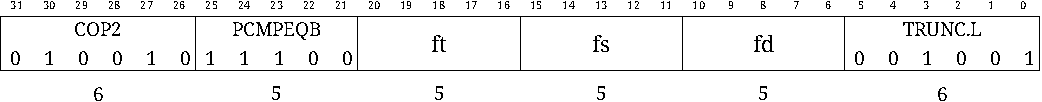
\includegraphics{ins-PCMPEQB} \\
  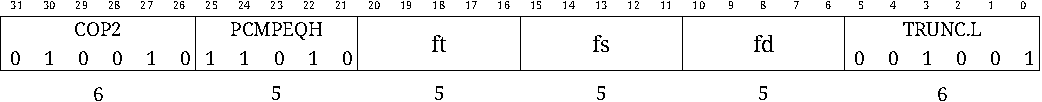
\includegraphics{ins-PCMPEQH} \\
  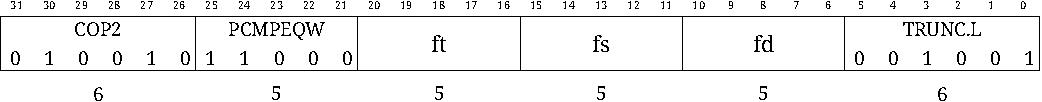
\includegraphics{ins-PCMPEQW} \\
  \instructionbody{PCMPEQB fd,fs,ft \narrownewline PCMPEQH fd,fs,ft \narrownewline PCMPEQW fd,fs,ft}
  {字节整数包的各元素是否相等}
  {这三条指令执行对第一个和第二个操作数中的整数包的各元素逐个进行相等比较操作:
  如果一对数据元素相等,则目标操作数的相应数据元素所有位皆设为1,否则全置为0。
  PCMPEQB指令用于比较第一和第二操作数的字节元素;
  PCMPEQH指令用于比较第一和第二操作数的半字元素;
  PCMPEQW指令用于比较第一和第二操作数的字元素。}
  {PCMPEQB \narrownewline
  fd[ 7..0 ] $\leftarrow$ fs[ 7..0 ] == ft[ 7..0 ] ? FFH : 0; \narrownewline
  * continue comparison of 2nd through 7th bytes in fs and ft * \narrownewline
  fd[63..56] $\leftarrow$ fs[63..56] == ft[63..56] ? FFH : 0; \narrownewline \narrownewline
  PCMPEQH \narrownewline
  fd[15..0 ] $\leftarrow$ fs[15..0 ] == ft[15..0 ] ? FFFFH : 0; \narrownewline
  * continue comparison of 2nd and 3rd halfwords in fs and ft * \narrownewline
  fd[63..48] $\leftarrow$ fs[63..48] == ft[63..48] ? FFFFH : 0; \narrownewline \narrownewline
  PCMPEQW \narrownewline
  fd[31..0 ] $\leftarrow$ fs[31..0 ] == ft[31..0 ] ? FFFFFFFFH : 0; \narrownewline
  fd[63..32] $\leftarrow$ fs[63..32] == ft[63..32] ? FFFFFFFFH : 0;}
  {无。}
\end{instructionblk}

\subsection{PEXTRH (半字抽取操作)}

\begin{instructionblk}
  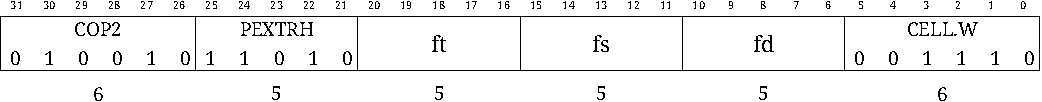
\includegraphics{ins-PEXTRH} \\
  \instructionbody{PEXTRH fd,fs,ft}
  {抽取指定的半字到目的寄存器}
  {该指令复制由第一个操作数的半字到目的操作数,
  该半字的位置为第二个操作数的低两位决定指定的。
  目的操作数的三个高位半字被清零。}
  {PEXTRH \narrownewline
  SEL $\leftarrow$ ft AND 3H; \narrownewline
  TEMP$\leftarrow$ fs >> (SEL * 16); \narrownewline
  fd[15..0 ] $\leftarrow$ TEMP[15..0 ]; \narrownewline
  fd[63..16] $\leftarrow$ 00000000H;}
  {无。}
\end{instructionblk}

\subsection{PINSRH (半字插入操作)}

\begin{instructionblk}
  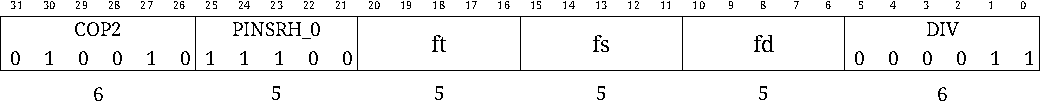
\includegraphics{ins-PINSRHo} \\
  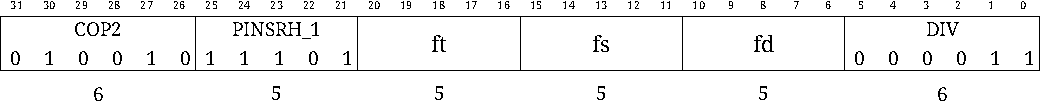
\includegraphics{ins-PINSRHi} \\
  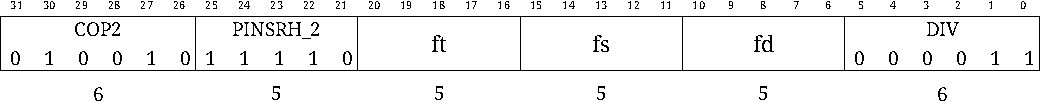
\includegraphics{ins-PINSRHii} \\
  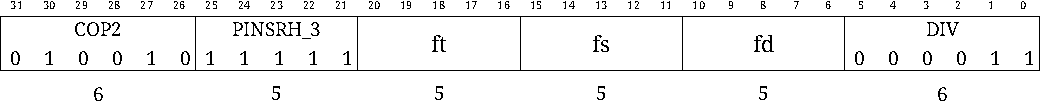
\includegraphics{ins-PINSRHiii} \\
  \instructionbody
  {PINSRH\_0 fd,fs,ft \narrownewline PINSRH\_1 fd,fs,ft \narrownewline PINSRH\_2 fd,fs,ft \narrownewline PINSRH\_3 fd,fs,ft}
  {}
  {复制第二个操作数的低位半字,插入到第一个操作数的
  指定位置,第一个操作数的其他半字保持不变,并将结果存入目的寄存器。}
  {PINSRH\_0 \narrownewline
  MASK$\leftarrow$ 000000000000FFFFH; \narrownewline
  fd  $\leftarrow$ (fs AND NOT MASK) OR ((ft << (0 * 16)) AND MASK); \narrownewline
  PINSRH\_1 \narrownewline
  MASK$\leftarrow$ 00000000FFFF0000H; \narrownewline
  fd  $\leftarrow$ (fs AND NOT MASK) OR ((ft << (1 * 16)) AND MASK); \narrownewline
  PINSRH\_2 \narrownewline
  MASK$\leftarrow$ 0000FFFF00000000H; \narrownewline
  fd  $\leftarrow$ (fs AND NOT MASK) OR ((ft << (2 * 16)) AND MASK); \narrownewline
  PINSRH\_3 \narrownewline
  MASK$\leftarrow$ FFFF000000000000H; \narrownewline
  fd  $\leftarrow$ (fs AND NOT MASK) OR ((ft << (3 * 16)) AND MASK);}
  {无。}
\end{instructionblk}

\subsection{PMADDHW (有符号整数包-半字到字-乘加运算)}

\begin{instructionblk}
  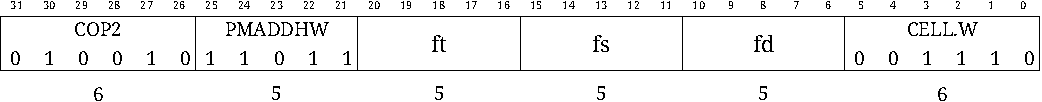
\includegraphics{ins-PMADDHW} \\
  \instructionbody{PMADDHW fd,fs,ft}
  {有符号半字整数包先乘后加,结果为字整数包类型}
  {该指令的具体操作为:首先将第一个操作数的四个有符号半字相乘分别与第二个操作数
  的相应有符号半字相乘,临时结果是四个有符号字。前两个字和后两个字分别后相加,
  结果存储在目的操作数。因为字整数被用来存储半字乘加的结果,一般而言,溢出不会发生。
  PMADDHW指令的溢出截断只会在一种情形下生效:当在一个操作组的两对半字,都是 8000H 时。
  在这种情况下,乘加的结果将会被截断为 80000000H。}
  {PMADDHW \narrownewline
  fd[31..0 ] $\leftarrow$ (fs[15..0 ] * ft[15..0 ]) + (fs[31..16] * ft[31..16]); \narrownewline
  fd[63..32] $\leftarrow$ (fs[47..32] * ft[47..32]) + (fs[63..48] * ft[63..48]);}
  {无。}
\end{instructionblk}

\subsection{PMAXSH/PMINSH (有符号半字整数包极值运算)}

\begin{instructionblk}
  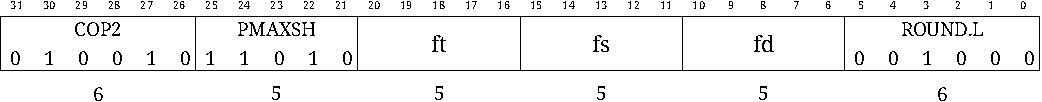
\includegraphics{ins-PMAXSH} \\
  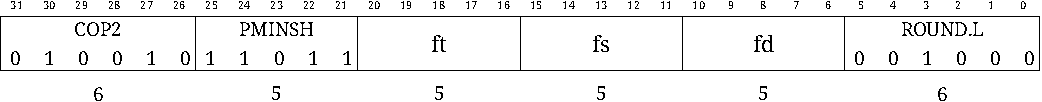
\includegraphics{ins-PMINSH} \\
  \instructionbody{PMAXSH fd,fs,ft \narrownewline PMINSH fd,fs,ft}
  {对两个有符号半字整数包的四对半字分别求极值。}
  {这两条指令对第一个操作数和第二个操作数的四对
  有符号半字分别求最大最小值,并将结果存入目的寄存器。}
  {PMAXSH \narrownewline
  fd[15..0 ] $\leftarrow$ max(fs[15..0 ], ft[15..0 ]); /* 有符号比较 */ \narrownewline
  * 对第二和第三个半字重复以上操作 \narrownewline
  fd[63..48] $\leftarrow$ max(fs[63..48], ft[63..48]); \narrownewline \narrownewline
  PMINSH \narrownewline
  fd[15..0 ] $\leftarrow$ min(fs[15..0 ], ft[15..0 ]); /* 有符号比较 */ \narrownewline
  * 对第二和第三个半字重复以上操作 \narrownewline
  fd[63..48] $\leftarrow$ min(fs[63..48], ft[63..48]);}
  {无。}
\end{instructionblk}

\subsection{PMAXUB/PMINUB (无符号字节整数包极值运算)}

\begin{instructionblk}
  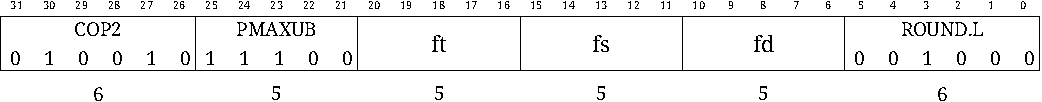
\includegraphics{ins-PMAXUB} \\
  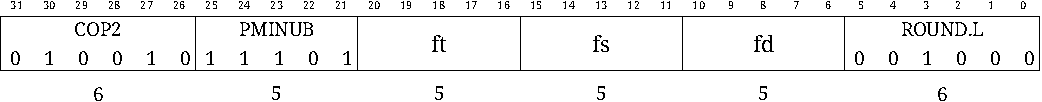
\includegraphics{ins-PMINUB} \\
  \instructionbody{PMAXUB fd,fs,ft \narrownewline PMINUB fd,fs,ft}
  {对两个无符号字节整数包的八对字节整数分别求极值。}
  {这两条指令对第一个操作数和第二个操作数的八对
  无符号字节整数分别求最大最小值,并将结果存入目的寄存器。}
  {PMAXUB \narrownewline
  fd[ 7..0 ] $\leftarrow$ max(fs[ 7..0 ], ft[ 7..0 ]); /* 无符号比较 */ \narrownewline
  * 对第二到第七个字节重复以上操作 * \narrownewline
  fd[63..56] $\leftarrow$ max(fs[63..56], ft[63..56]); \narrownewline \narrownewline
  PINXUB \narrownewline
  fd[ 7..0 ] $\leftarrow$ min(fs[ 7..0 ], ft[ 7..0 ]); /* 无符号比较 */ \narrownewline
  * 对第二到第七个字节重复以上操作 * \narrownewline
  fd[63..56] $\leftarrow$ min(fs[63..56], ft[63..56]);}
  {无。}
\end{instructionblk}

\subsection{PMOVMSKB (字节掩码移动操作)}

\remark{two operands!}
\begin{instructionblk}
  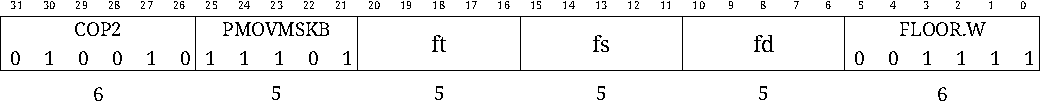
\includegraphics{ins-PMOVMSKB} \\
  \instructionbody{PMOVMSKB fd,fs}
  {将字节整数包的8个字节掩码归并到一个字节上。}
  {该指令是将第一个操作数(一个64位的字节整数包)的八个字节的
  最高位(即掩码位)归并且存储在目标操作数的低字节中。}
  {PMOVMSKB \narrownewline
  fd[0] $\leftarrow$ fs[ 7]; \narrownewline
  fd[1] $\leftarrow$ fs[15]; \narrownewline
  * 对第三到第七个字节重复以上操作 * \narrownewline
  fd[7] $\leftarrow$ fs[63]; \narrownewline
  fd[63..8 ] $\leftarrow$ 00000000000000H;}
  {无。}
\end{instructionblk}

\subsection{PMULHUH (无符号半字整数包乘:高位结果)}

\begin{instructionblk}
  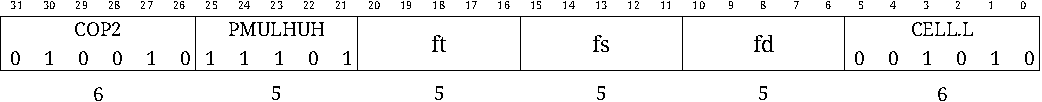
\includegraphics{ins-PMULHUH} \\
  \instructionbody{PMULHUH fd,fs,ft}
  {无符号半字整数包的乘法运算,并存储高位结果。}
  {该指令执行无符号半字整数包的乘法运算,并将四个乘法结果的高半字结果存储
  到目的寄存器中。}
  {PMULHUH \narrownewline
  fd[15..0 ] $\leftarrow$ (fs[15..0 ] * ft[15..0 ])[31..16]; /* 无符号乘 */ \narrownewline
  fd[31..16] $\leftarrow$ (fs[31..16] * ft[31..16])[31..16]; \narrownewline
  fd[47..32] $\leftarrow$ (fs[47..32] * ft[47..32])[31..16]; \narrownewline
  fd[63..48] $\leftarrow$ (fs[63..48] * ft[63..48])[31..16];}
  {无。}
\end{instructionblk}

\subsection{PMULHH/PMULLH (有符号半字整数包乘:高位、低位结果)}

\begin{instructionblk}
  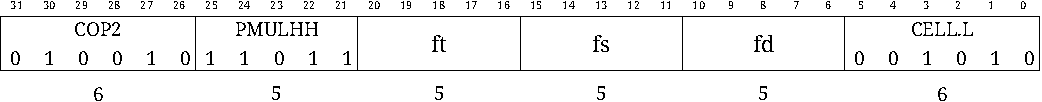
\includegraphics{ins-PMULHH} \\
  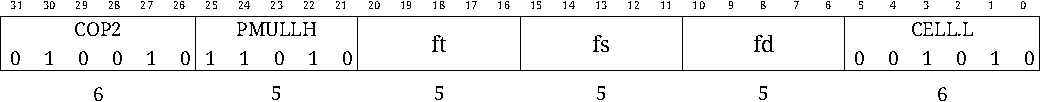
\includegraphics{ins-PMULLH} \\
  \instructionbody{PMULHH fd,fs,ft \narrownewline PMULLH fd,fs,ft}
  {有符号半字整数包的乘法运算,并分别存储高位、低位结果。}
  {这两条指令执行无符号半字整数包的乘法运算,并分别将四个乘法结果的高半字
  或者低半字结果存储到目的寄存器中。}
  {PMULHH \narrownewline
  fd[15..0 ] $\leftarrow$ (fs[15..0 ] * ft[15..0 ])[31..16]; /* 有符号乘 */ \narrownewline
  fd[31..16] $\leftarrow$ (fs[31..16] * ft[31..16])[31..16]; \narrownewline
  fd[47..32] $\leftarrow$ (fs[47..32] * ft[47..32])[31..16]; \narrownewline
  fd[63..48] $\leftarrow$ (fs[63..48] * ft[63..48])[31..16]; \narrownewline \narrownewline
  PMULLH \narrownewline
  fd[15..0 ] $\leftarrow$ (fs[15..0 ] * ft[15..0 ])[15..0 ]; /* 有符号乘 */ \narrownewline
  fd[31..16] $\leftarrow$ (fs[31..16] * ft[31..16])[15..0 ]; \narrownewline
  fd[47..32] $\leftarrow$ (fs[47..32] * ft[47..32])[15..0 ]; \narrownewline
  fd[63..48] $\leftarrow$ (fs[63..48] * ft[63..48])[15..0 ];}
  {无。}
\end{instructionblk}

\subsection{PMULUW (无符号字整数包乘)}

\begin{instructionblk}
  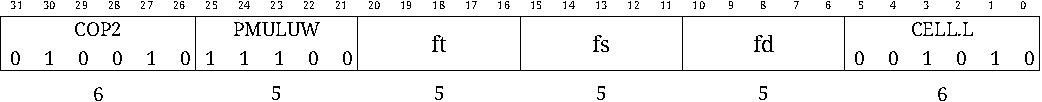
\includegraphics{ins-PMULUW} \\
  \instructionbody{PMULUW fd,fs,ft}
  {执行无符号字整数包乘法运算,溢出采用截断模式。}
  {该指令执行无符号字整数包乘法运算,具体操作为将第一个操作数的低字整数与
  第二个操作数低字整数相乘,并将无符号整数结果存储 64 的目的操作数。源操作数和
  结果都是无符号整数。如果结果太大,在64位上溢出,则将会被截断,只有低64位写入
  到目标中(即进位被忽略)。}
  {PMULUW \narrownewline
  fd[63..0] $\leftarrow$ fs[31..0] * ft[31..0];}
  {无。}
\end{instructionblk}

\subsection{PASUBUB (无符号字节包 绝对差值运算)}

\begin{instructionblk}
  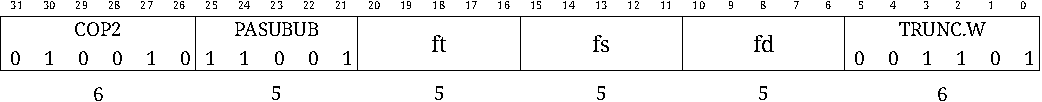
\includegraphics{ins-PASUBUB} \\
  \instructionbody{PASUBUB fd,fs,ft}
  {计算无符号字节整数包的对应元素的绝对差值。}
  {PSADBH指令计算两个无符号字节整数包的八对字节整数
  的绝对差值,即差的绝对值,物理意义一般就是距离。}
  {PASUBUB \narrownewline
  fd[ 7..0 ] $\leftarrow$ ABS(fs[ 7..0 ] - ft[ 7..0 ]); \narrownewline
  * repeat operation for bytes 2 through 6 * \narrownewline
  fd[63..56] $\leftarrow$ ABS(fs[63..56] - ft[63..56]);}
  {无。}
\end{instructionblk}

\subsection{BIADD (无符号字节包内部和)}

\begin{instructionblk}
  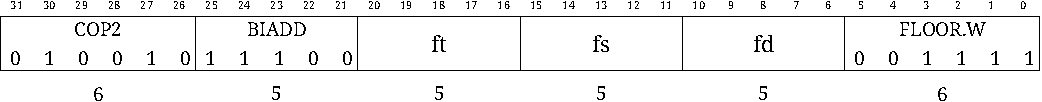
\includegraphics{ins-BIADD} \\
  \instructionbody{BIADD fd,fs}
  {计算无符号字节包内所有字节整数的和,结果为一个半字整数。}
  {PSADBH指令计算第一个操作数(一个无符号字节整数包)
  的八个字节整数的和。结果是一个无符号的半字整数,并
  存储在目的操作数的低字位置,目标操作数的其余字节都将
  被清零。}
  {BIADD \narrownewline
  fd[15..0 ] $\leftarrow$ SUM(fs[7..0], fs[15..8], ..., fs[63..56]); \narrownewline
  fd[63..16] $\leftarrow$ 000000000000H;}
  {无。}
\end{instructionblk}

\subsection{PSHUFH (半字包换位操作)}

\begin{instructionblk}
  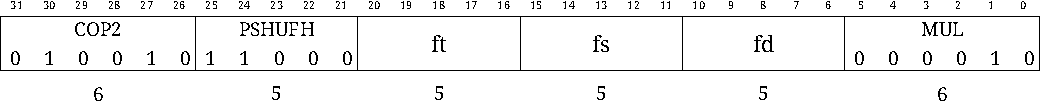
\includegraphics{ins-PSHUFH} \\
  \instructionbody{PSHUFH fd,fs,ft}
  {将半字包按指定的位置换位并复制到目的寄存器。}
  {该指令的具体操作是将第一个操作数的各个半字按
  第二个操作数给出的位置插入到目的操作数中去。
  第二个操作数对每个半字位置用两位(2 bits)来编码。具体编码为 --- $00_2$:
  半字$_0$; $01_2$: 半字$_1$; $10_2$: 半字$_2$; $11_2$: 半字$_3$;。
  注意,该指令允许在一个半字被复制到目的操作数的多个位置。}
  {PSHUFH \narrownewline
  fd[15..0 ] $\leftarrow$ (fs >> (ft[1..0] * 16))[15..0] \narrownewline
  fd[31..16] $\leftarrow$ (fs >> (ft[3..2] * 16))[15..0] \narrownewline
  fd[47..32] $\leftarrow$ (fs >> (ft[5..4] * 16))[15..0] \narrownewline
  fd[63..48] $\leftarrow$ (fs >> (ft[7..6] * 16))[15..0]}
  {无。}
\end{instructionblk}

\subsection{PSLLH/PSLLW (整数包逻辑左移位)}

\begin{instructionblk}
  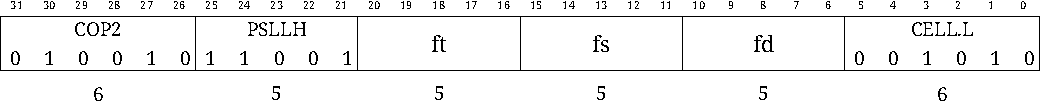
\includegraphics{ins-PSLLH} \\
  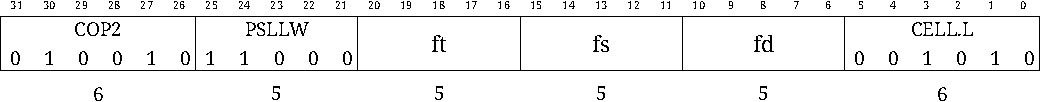
\includegraphics{ins-PSLLW} \\
  \instructionbody{PSLLH fd,fs,ft \narrownewline PSLLW fd,fs,ft}
  {半字或字整数包的逻辑左移位运算。}
  {这两条指令分别对第一个操作数中的半字或字元素进行逻辑左移位运算,并
  将结果存储在目的寄存器中。
  移动的位数由第二个操作数的低7位指定。移位采用逻辑移位方式,即当数据元素
  被左移时,空出的低序位被零填充。如果移位值大于15(半字),31
  (字),则移位结果为0。}
  {PSLLH \narrownewline
  IF (ft[6..0 ] > 15) \narrownewline
  THEN \narrownewline
  \mbox{\hspace{.5cm}} fd[64..0 ] $\leftarrow$ 0000000000000000H \narrownewline
  ELSE \narrownewline
  \mbox{\hspace{.5cm}} fd[15..0 ] $\leftarrow$ ZeroExtend(fs[15..0 ] << ft[6..0]); \narrownewline
  \mbox{\hspace{.5cm}} * repeat shift operation for 2nd and 3rd words *; \narrownewline
  \mbox{\hspace{.5cm}} fd[63..48] $\leftarrow$ ZeroExtend(fs[63..48] << ft[6..0]); \narrownewline
  FI; \narrownewline \narrownewline
  PSLLW \narrownewline
  IF (ft[6..0 ] > 31) \narrownewline
  THEN \narrownewline
  \mbox{\hspace{.5cm}} fd[64..0 ] $\leftarrow$ 0000000000000000H \narrownewline
  ELSE \narrownewline
  \mbox{\hspace{.5cm}} fd[31..0 ] $\leftarrow$ ZeroExtend(fs[31..0 ] << ft[6..0]); \narrownewline
  \mbox{\hspace{.5cm}} fd[63..32] $\leftarrow$ ZeroExtend(fs[63..32] << ft[6..0]); \narrownewline
  FI;}
  {无。}
\end{instructionblk}

\subsection{PSRAH/PSRAW (整数包算数右移位)}

\begin{instructionblk}
  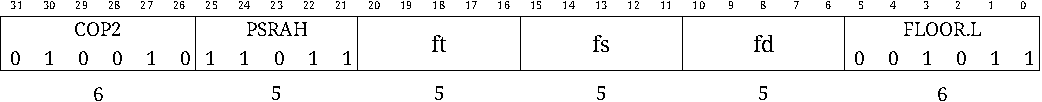
\includegraphics{ins-PSRAH} \\
  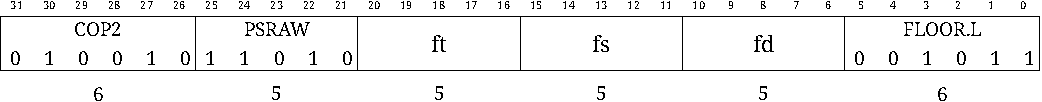
\includegraphics{ins-PSRAW} \\
  \instructionbody{PSRAH fd,fs,ft \narrownewline PSRAW fd,fs,ft}
  {半字或字整数包的算数右移位运算。}
  {这两条指令分别对第一个操作数中的半字或字元素进行算数右移位运算,并
  将结果存储在目的寄存器中。
  移动的位数由第二个操作数的低7位指定。移位采用算数移位方式,即当数据元素
  被右移时,空出的高序位由初始的符号位的值填充。如果移位值大于15(半字),31
  (字),则移位结果为各位都是了元素符号位的初始值。}
  {PSRAH \narrownewline
  IF (ft[6..0] > 16) THEN ft[6..0] $\leftarrow$ 16; \narrownewline
  fd[15..0 ] $\leftarrow$ SignExtend(fs[15..0 ] >> ft[6..0]); \narrownewline
  * repeat shift operation for 2nd and 3rd halfwords *; \narrownewline
  fd[63..48] $\leftarrow$ SignExtend(fs[63..48] >> ft[6..0]); \narrownewline \narrownewline
  PSRAW \narrownewline
  IF (ft[6..0 ] > 31) THEN ft[6..0] $\leftarrow$ 32; \narrownewline
  fd[31..0 ] $\leftarrow$ SignExtend(fs[31..0 ] >> ft[6..0]); \narrownewline
  fd[63..32] $\leftarrow$ SignExtend(fs[63..32] >> ft[6..0]);}
  {无。}
\end{instructionblk}

\subsection{PSRLH/PSRLW (整数包逻辑右移位)}

\begin{instructionblk}
  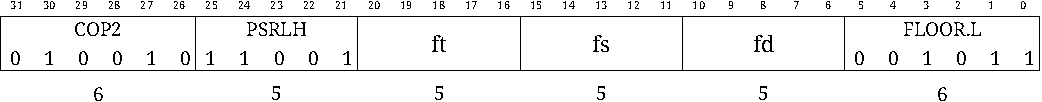
\includegraphics{ins-PSRLH} \\
  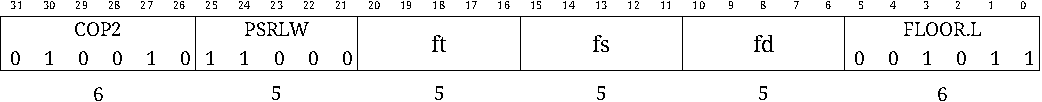
\includegraphics{ins-PSRLW} \\
  \instructionbody{PSRLH fd,fs,ft \narrownewline PSRLW fd,fs,ft}
  {半字或字整数包的逻辑右移位运算。}
  {这两条指令分别对第一个操作数中的半字或字元素进行逻辑右移位运算,并
  将结果存储在目的寄存器中。
  移动的位数由第二个操作数的低7位指定。移位采用逻辑移位方式,即当数据元素
  被右移时,空出的高序位将被零填充。如果移位值大于15(半字),31
  (字),则移位结果为0。}
  {PSRLH \narrownewline
  IF (ft[6..0] > 15) \narrownewline
  THEN \narrownewline
  \mbox{\hspace{.5cm}} fd[64..0 ] $\leftarrow$ 0000000000000000H \narrownewline
  ELSE \narrownewline
  \mbox{\hspace{.5cm}} fd[15..0 ] $\leftarrow$ ZeroExtend(fs[15..0 ] >> ft[6..0]); \narrownewline
  \mbox{\hspace{.5cm}} * repeat shift operation for 2nd and 3rd halfwords *; \narrownewline
  \mbox{\hspace{.5cm}} fd[63..48] $\leftarrow$ ZeroExtend(fs[63..48] >> ft[6..0]); \narrownewline
  FI; \narrownewline \narrownewline
  PSRLW \narrownewline
  IF (ft[6..0] > 31) \narrownewline
  THEN \narrownewline
  \mbox{\hspace{.5cm}} fd[64..0 ] $\leftarrow$ 0000000000000000H \narrownewline
  ELSE \narrownewline
  \mbox{\hspace{.5cm}} fd[31..0 ] $\leftarrow$ ZeroExtend(fs[31..0 ] >> ft[6..0]); \narrownewline
  \mbox{\hspace{.5cm}} fd[63..32] $\leftarrow$ ZeroExtend(fs[63..32] >> ft[6..0]); \narrownewline
  FI;}
  {无。}
\end{instructionblk}

\subsection{PSUBB/PSUBH/PSUBW/PSUBD (整数包减)}

\begin{instructionblk}
  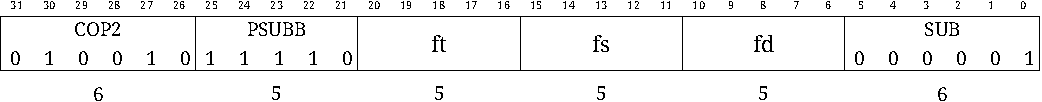
\includegraphics{ins-PSUBB} \\
  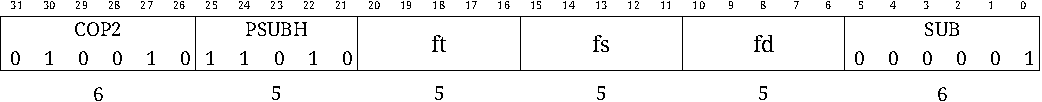
\includegraphics{ins-PSUBH} \\
  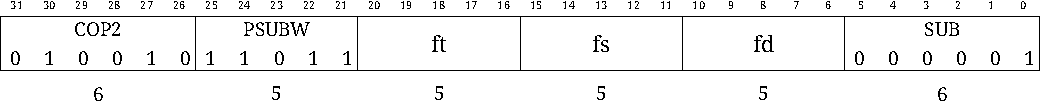
\includegraphics{ins-PSUBW} \\
  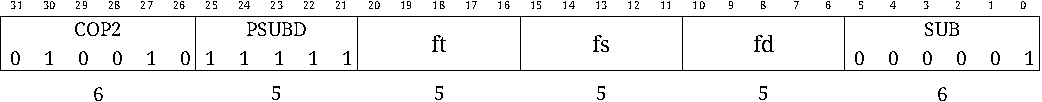
\includegraphics{ins-PSUBD} \\
  \instructionbody{PSUBB fd,fs,ft \narrownewline PSUBH fd,fs,ft \narrownewline
  PSUBW fd,fs,ft \narrownewline PSUBD fd,fs,ft}
  {使用截断模式执行各种类型整数包相减运算。}
  {这四条指令用于执行各种整数包的减法操作: 它们分别将第一个和第二个操作寄存器的
  对应位置的各个操作数(依照指令给定的数据类型)相减,并将结果存储在目标操作数中。
  溢出处理为截断模式。 比如说, PSUBB指令的具体操作是将第一个和第二个操作寄存器
  对应的 8 个字节整数相减。当任何一个减法结果太大,即在第9位溢出时,只有低 8
  位结果将被写入到目标操作数(进位被忽略)。其他三个指令与PSUBB类似。
  
  注意,这四条包减法指令既可以应用于无符号,也可以应用于(采用2的补码
  表示法的)有符号整数包。 为了避免溢出或进位情况的发生,软件必须控制操作数的范围。}
  {PSUBB \narrownewline
  fd[ 7..0 ]  $\leftarrow$ fs[ 7..0 ] - ft[ 7..0 ]; \narrownewline
  * repeat subtract operation for 2nd through 7th byte *; \narrownewline
  fd[63..56] $\leftarrow$ fs[63..56] - ft[63..56]; \narrownewline \narrownewline
  PSUBH \narrownewline
  fd[15..0 ] $\leftarrow$ fs[15..0 ] - ft[15..0 ]; \narrownewline
  * repeat subtract operation for 2nd and 3rd halfword *; \narrownewline
  fd[63..48] $\leftarrow$ fs[63..48] - ft[63..48]; \narrownewline \narrownewline
  PSUBW \narrownewline
  fd[31..0 ] $\leftarrow$ fs[31..0 ] - ft[31..0 ]; \narrownewline
  fd[63..32] $\leftarrow$ fs[63..32] - ft[63..32]; \narrownewline \narrownewline
  PSUBD \narrownewline
  fd[63..0] $\leftarrow$ fs[63..0] - ft[63..0];}
  {无。}
\end{instructionblk}

\subsection{PSUBSB/PSUBSH (有符号整数包减)}

\begin{instructionblk}
  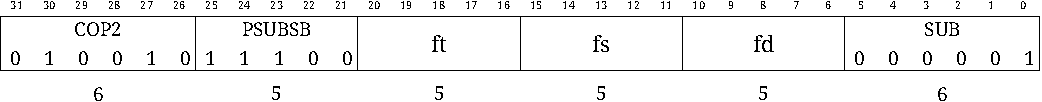
\includegraphics{ins-PSUBSB} \\
  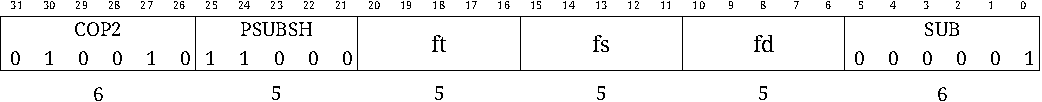
\includegraphics{ins-PSUBSH} \\
  \instructionbody{PSUBSB fd,fs,ft \narrownewline PSUBSH fd,fs,ft}
  {有符号整数包减法指令。}
  {这两条指令用于执行各种有符号整数包的减法操作: 它们分别将第一个和第二个操作寄存器的
  对应位置的各个操作数(依照指令给定的数据类型)相加,并将结果存储在目标操作数中。
  溢出处理采用有符号饱和模式。 这些指令的操作数皆为 64 位。

  PSUBSB 指令的具体操作是将第一个和第二个操作寄存器
  对应的 8 个有符号字节整数相减。当任何一个减法结果太大或太小,
  超出了一个有符号字节的整数范围(即大于 7FH 或少于
  80H),则对应的饱和值7FH或80H,将被写入目的操作数。
  相应的, PSUBSH 指令操作有符号半字整数。当一个
  半字相减的结果超出了有符号半字整数范围时(即大于
  7FFFH或小于8000H),则7FFFH或8000H的作为饱和值,将写入目标操作数。}
  {PSUBSB \narrownewline
  fd[ 7..0 ]  $\leftarrow$ SaturateToSignedByte(fs[ 7..0 ] - ft[ 7..0 ]) ; \narrownewline
  * repeat subtract operation for 2nd through 7th bytes *; \narrownewline
  fd[63..56] $\leftarrow$ SaturateToSignedByte(fs[63..56] - ft[63..56]); \narrownewline \narrownewline
  PSUBSH \narrownewline
  fd[15..0 ] $\leftarrow$ SaturateToSignedHalfword(fs[15..0 ] - ft[15..0 ]); \narrownewline
  * repeat subtract operation for 2nd and 4th halfwords *; \narrownewline
  fd[63..48] $\leftarrow$ SaturateToSignedHalfword(fs[63..48] - ft[63..48]);}
  {无。}
\end{instructionblk}

\subsection{PSUBUSB/PSUBUSH (无符号整数包减)}

\begin{instructionblk}
  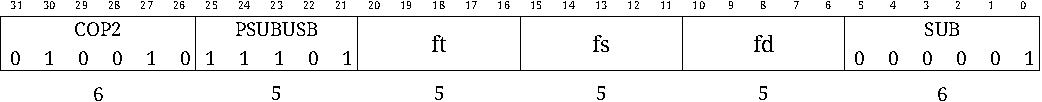
\includegraphics{ins-PSUBUSB} \\
  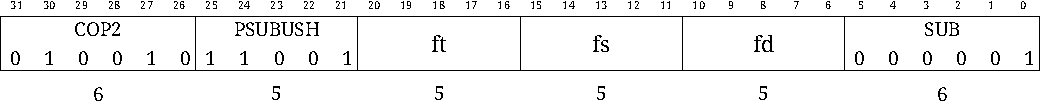
\includegraphics{ins-PSUBUSH} \\
  \instructionbody{PSUBUSB fd,fs,ft \narrownewline PSUBUSH fd,fs,ft}
  {无符号整数包减法运算。}
  {这两条指令用于执行各种无符号整数包减操作: 它们分别将第一个和第二个操作寄存器的
  对应位置的各个操作数(依照指令给定的数据类型)相减,并将结果存储在目标操作数中。
  溢出处理采用无符号饱和模式。

  PSUBUSB 指令的具体操作是将第一个和第二个操作寄存器
  对应的 8 个无符号字节整数相减。当任何一个减法结果太小,
  超出了一个无符号字节的整数范围(即小于 00H),
  则 00H 将作为饱和值写入目的操作数。
  相应的, PSUBUSH 指令操作无符号半字整数。当一个
  半字相减的结果超出了无符号半字整数范围时(即小于
  0000H),则 0000H 将作为饱和值将写入目标操作数。}
  {PSUBUSB \narrownewline
  fd[ 7..0 ]  $\leftarrow$ SaturateToUnsignedByte(fs[ 7..0 ] - ft[ 7..0 ]) ; \narrownewline
  * repeat add operation for 2nd through 7th bytes *; \narrownewline
  fd[63..56] $\leftarrow$ SaturateToUnsignedByte(fs[63..56] - ft[63..56]); \narrownewline \narrownewline
  PSUBUSH \narrownewline
  fd[15..0 ] $\leftarrow$ SaturateToUnsignedHalfword(fs[15..0 ] - ft[15..0 ]); \narrownewline
  * repeat add operation for 2nd and 3rd halfwords *; \narrownewline
  fd[63..48] $\leftarrow$ SaturateToUnsignedHalfword(fs[63..48] - ft[63..48]);}
  {无。}
\end{instructionblk}

\subsection{PUNPCKHBH/PUNPCKHHW/PUNPCKHWD (高位拆包)}

\begin{instructionblk}
  \includegraphics{ins-PUNPCKHBH} \\
  \includegraphics{ins-PUNPCKHHW} \\
  \includegraphics{ins-PUNPCKHWD} \\
  \instructionbody{PUNPCKHBH fd,fs,ft \narrownewline PUNPCKHHW fd,fs,ft \narrownewline PUNPCKHWD fd,fs,ft}
  {不同类型整数包的高位拆包操作。}
  {这三条指令用于对不同类型的整数包的高位拆包。其具体操作为将
  第一个操作数和第二个操作数的高位(32位)取出,并拆分成给定的
  宽度(PUNPCKHBH:字节; PUNPCKHHW:半字; PUNPCKHWD:字),然后按交替的顺序
  合并到目的寄存器中。所有低位信息被忽略。更具体的
  拆包后合并的位对应关系可参见操作部分。
  
  如果第二个操作数值为0, 则这些指令的实质结果是分别将高位的四个字节
  转换为四个半字,高位的两个半字为两个字,高位的一个字为双字(都是无符号类型)。}
  {PUNPCKHBH \narrownewline
  fd[ 7..0 ] $\leftarrow$ fs[39..32]; \narrownewline
  fd[15..8 ] $\leftarrow$ ft[39..32]; \narrownewline
  fd[23..16] $\leftarrow$ fs[47..0 ]; \narrownewline
  fd[31..24] $\leftarrow$ ft[47..0 ]; \narrownewline
  fd[39..32] $\leftarrow$ fs[55..48]; \narrownewline
  fd[47..0 ] $\leftarrow$ ft[55..48]; \narrownewline
  fd[55..48] $\leftarrow$ fs[63..56]; \narrownewline
  fd[63..56] $\leftarrow$ ft[63..56]; \narrownewline \narrownewline
  PUNPCKHHW \narrownewline
  fd[15..0 ] $\leftarrow$ fs[47..32]; \narrownewline
  fd[31..16] $\leftarrow$ ft[47..32]; \narrownewline
  fd[47..32] $\leftarrow$ fs[63..48]; \narrownewline
  fd[63..48] $\leftarrow$ ft[63..48]; \narrownewline \narrownewline
  PUNPCKHWD \narrownewline
  fd[31..0 ] $\leftarrow$ fs[63..32] \narrownewline
  fd[63..32] $\leftarrow$ ft[63..32];}
  {无。}
\end{instructionblk}

\subsection{PUNPCKLBH/PUNPCKLHW/PUNPCKLWD (低位拆包)}

\begin{instructionblk}
  \includegraphics{ins-PUNPCKLBH} \\
  \includegraphics{ins-PUNPCKLHW} \\
  \includegraphics{ins-PUNPCKLWD} \\
  \instructionbody{PUNPCKLBH fd,fs,ft \narrownewline PUNPCKLHW fd,fs,ft \narrownewline PUNPCKLWD fd,fs,ft}
  {不同类型整数包的低位拆包操作。}
  {这三条指令用于对不同类型的整数包的低位拆包。其具体操作为将
  第一个操作数和第二个操作数的低位(32位)取出,并拆分成给定的
  宽度(PUNPCKHBH:字节; PUNPCKHHW:半字; PUNPCKHWD:字),然后按交替的顺序
  合并到目的寄存器中。所有低位信息被忽略。更具体的
  拆包后合并的位对应关系可参见操作部分。
  
  如果第二个操作数值为0, 则这些指令的实质结果是分别将低位的四个字节
  转换为四个半字,低位的两个半字为两个字,低位的一个字为双字(都是无符号类型)。}
  {PUNPCKLBH \narrownewline
  fd[63..56] $\leftarrow$ ft[31..24]; \narrownewline
  fd[55..48] $\leftarrow$ fs[31..24]; \narrownewline
  fd[47..0 ] $\leftarrow$ ft[23..16]; \narrownewline
  fd[39..32] $\leftarrow$ fs[23..16]; \narrownewline
  fd[31..24] $\leftarrow$ ft[15..8 ]; \narrownewline
  fd[23..16] $\leftarrow$ fs[15..8 ]; \narrownewline
  fd[15..8 ] $\leftarrow$  ft[ 7..0 ]; \narrownewline
  fd[ 7..0 ]  $\leftarrow$ fs[ 7..0 ]; \narrownewline \narrownewline
  PUNPCKLHW \narrownewline
  fd[63..48] $\leftarrow$ ft[31..16]; \narrownewline
  fd[47..32] $\leftarrow$ fs[31..16]; \narrownewline
  fd[31..16] $\leftarrow$ ft[15..0 ]; \narrownewline
  fd[15..0 ] $\leftarrow$ fs[15..0 ]; \narrownewline \narrownewline
  PUNPCKLWD \narrownewline
  fd[63..32] $\leftarrow$ ft[31..0 ]; \narrownewline
  fd[31..0 ] $\leftarrow$ fs[31..0 ];}
  {无。}
\end{instructionblk}
